\documentclass{standalone}
%% Show/hide steps for standalone work — edit this line:
\makeatletter\AtBeginDocument{\@buildstepset{1,2,3,4,5,6,7,8,9,10}}\makeatother
\usepackage{tikz}
\usetikzlibrary{intersections,calc}
\usepackage{amsmath}
\usepackage{hsbcommon}
\begin{document}
    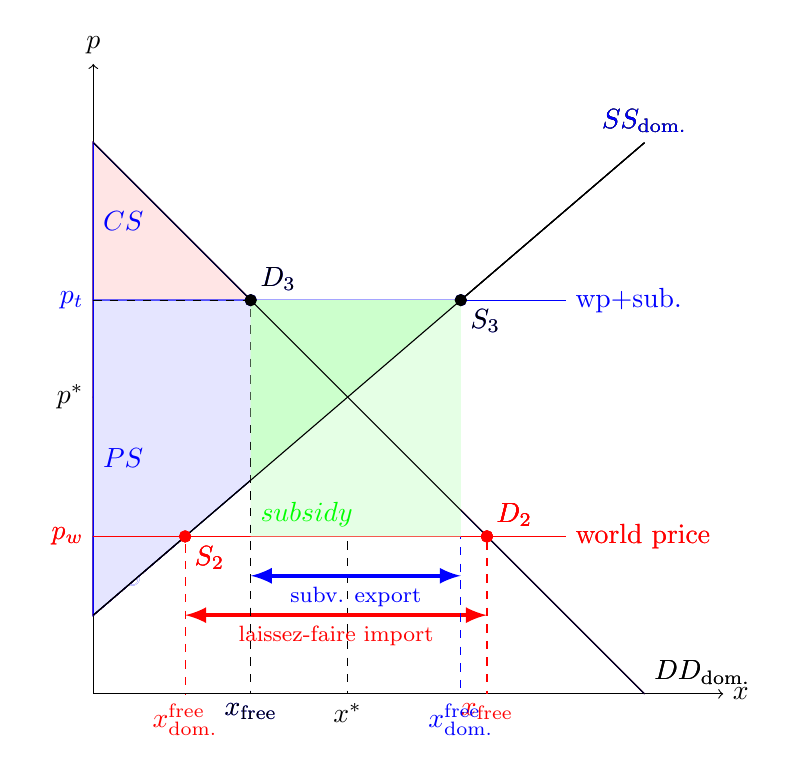
\begin{tikzpicture}
        \draw[->] (0,0) node[below] {\phantom{$X_mi$}} -- (8,0) node (Y) [right] {$x$};
        \draw[->] (0,0) node[left] {\phantom{$Y_mi$}} -- (0,8) node (i) [above] {$p$};
        
        \coordinate (A) at (0,7);
        \coordinate (B) at (7,0);
        \coordinate (E) at (0,1);
        \coordinate (F) at (7,7);
        
        \draw[name path=demand] plot [smooth] coordinates {(A) (B) };
        \node[above right] at (B) {$DD_{\text{dom.}}$};
        
        \draw[name path=supply] plot [smooth] coordinates {(E) (F)};
        \node[above] at (F) {$SS_{\text{dom.}}$};
           
        
        \path [name intersections={of=demand and supply,by=X}];

        \draw[dashed] (0, |- X) node [left] {$p^*$} -- (X) -- (X |-, 0)  node [below] {$x^*$}; 
    
        
        \draw[fill=red!10] (A) --  (X) --   (0, |- X) -- node[right] {$CS$} cycle;
        \draw[fill=blue!10] (E) --  (X) --   (0, |- X) -- node[right] {$PS$} cycle;
        \filldraw (X) node[right] {$D_1$} circle (2pt);

        \ifstep{1}{
\begin{scope}[color=red]



            \draw[name path=worldprice] (0,2) node[left] {$p_w$} -- (6,2) node[right] {world price};

            

            \path[name intersections={of=demand and worldprice,by=Y}];
            \path[name intersections={of=supply and worldprice,by=Z}];
            

            \draw[dashed] (0, |- Y) -- (Y) -- (Y |-, 0) node[below] {$x_ {\text{free}}$};
            \draw[dashed] (0, |- Z) -- (Z) -- (Z |-, 0) node[below] {$x_ {\text{dom.}}^{\text{free}}$};

            \draw[ultra thick,<->,>=latex] (Y |-, 1) -- node[below] {\footnotesize laissez-faire import} (Z |-, 1);
            
            \draw[fill=red!10] (A) --  (Y) --   (0, |- Y) -- node[right] {$CS$} cycle;
            
            \draw[draw=black] plot [smooth] coordinates {(E) (F)};
            \node[color= black, above] at (F) {$SS_{\text{dom.}}$};
            
            \draw[fill=blue!10] (E) --  (Z) --   (0, |- Z) -- node[color=blue, right] {$PS$} cycle;
            
            \draw[name path=demand] plot [smooth] coordinates {(A) (B) };
            \filldraw[color=black] (X) node[right] {$D_1$} circle (2pt);
                
            \filldraw (Z) node[below right] {$S_2$} circle (2pt);         
            \filldraw[red] (Y) node[above right] {$D_2$} circle (2pt);         

            
        \end{scope}
}


        \ifstep{2}{
\begin{scope}[color=blue]

            \draw[fill=white] (E) --  (Z) --   (0, |- Z) -- node[color=white, right] {$PS$} cycle;
            \fill[white] (A) --  (Y) --   (0, |- Y) -- node[right] {$CS$} cycle;
            \filldraw[red] (Y) node[above right] {$D_2$} circle (2pt);         
            
            \draw[name path=tariff] (0,5) node[left] {$p_t$} -- (6,5) node[right] {wp+sub.};

            \path[name intersections={of=demand and tariff,by=Y2}];
            \path[name intersections={of=supply and tariff,by=Z2}];
            
            \draw[fill=red!10] (A) --  (Y2) --   (0, |- Y2) -- node[right] {$CS$} cycle;
            \filldraw[black] (X) node[right] {$D_1$} circle (2pt);
            
            \draw[fill=blue!10] (E) --  (Z2) --   (0, |- Z2) -- node[right] {$PS$} cycle;
            

            \draw[dashed,name path=xfree] (0, |- Y2) -- (Y2) -- (Y2 |-, 0) node[below] {$x_{\text{free}}$};
            \draw[dashed] (0, |- Z2) -- (Z2) -- (Z2 |-, 0) node[below] {$x_ {\text{dom.}}^{\text{free}}$};
            
            \draw[ultra thick,<->,>=latex] (Y2 |-, 1.5) -- node[below] {\footnotesize subv. export} (Z2 |-, 1.5);
            
            \draw[name path=demand] plot [smooth] coordinates {(A) (B) };
            \draw[color=red, name path=worldprice] (0,2) node[left] {$p_w$} -- (6,2) node[right] {world price};
            
            \filldraw[red] (Z) node[below right] {$S_2$} circle (2pt);   
            
            \filldraw[color=black] (X) node[right] {$D_1$} circle (2pt);
            \filldraw (Y2) node[above right] {$D_3$} circle (2pt);         
            \filldraw (Z2) node[below right] {$S_3$} circle (2pt);             

            \draw[draw=black] plot [smooth] coordinates {(E) (F)};
            \node[above] at (F) {$SS_{\text{dom.}}$};
            
        \end{scope}
}

        
        \ifstep{3}{

            \fill[color=green!10] (Z2) -- (Y2) -- (Y2 |-,2) node[green, above right] {$subsidy$}  -- (Z2 |-, 2)  ;
            \draw[dashed,name path=xfree] (0, |- Y2) -- (Y2)-- (Y2 |-, 0) node[below] {$x_{\text{free}}$};
            \path[name intersections={of=xfree and supply,by=Y3}];
            \fill[color=green!20] (Z2) -- (Y2) -- (Y3);
            \draw[draw=black] plot [smooth] coordinates {(E) (F)};
            \draw[name path=demand] plot [smooth] coordinates {(A) (B) };
            \node[above right] at (B) {$DD_{\text{dom.}}$};            
            \filldraw (Y2) node[above right] {$D_3$} circle (2pt);         
            \filldraw (Z2) node[below right] {$S_3$} circle (2pt);        
            \filldraw[red] (Y) node[above right] {$D_2$} circle (2pt);     
            \filldraw[red] (Z) node[below right] {$S_2$} circle (2pt);   
            \filldraw[red] (Y) node[above right] {$D_2$} circle (2pt);         
        }

     
            
    \end{tikzpicture}
\end{document}